\svnkwsave{$RepoFile: siminos/baroclinic/intro.tex $}
\svnidlong {$HeadURL$}
{$LastChangedDate$}
{$LastChangedRevision$} {$LastChangedBy$}
\svnid{$Id$}

\chapter{Baroclinic flows}
\label{chap:baroclinic}

    \ifboyscout
To view just the project (without this line and the blog)
toggle the \texttt{boyscoutfalse} switch, towards the top of
\texttt{siminos/baroclinic/BrCv12.tex} file.
    \fi

\section{Introduction}
\label{s:intro}

    \SOA{Not really sure if it is the hardest one to understand. But I
    remembered it seem to distant to me the first time the concept was
    introduced to me.}
The concept of baroclinic instability is perhaps one of the harder ones
to grasp in geophysical fluid mechanics. However, it is also one of the
most fundamental concepts on this field, as it is the main driver for the
large scale circulations in the atmosphere and important circulations in
the ocean. It is by this mechanism that the atmosphere redistributes heat
from low latitudes to high latitudes, that it sustains synoptic weather
system and by which some oceanic eddies develop. Its importance can not
be overstated.

    \SOA{Here I am mostly speculating. However, this is the impression I
    have so far}
On the other hand, one could argue that the study of baroclinic flows
remains in its early stages. Although there exist a very well developed
linear theory for the onset of this type of instability, there still much
room to explore the nonlinear regimes. A way to approach this studies is
given by recent advances in the dynamical approaches to study of
turbulence\rf{science04,Waleffe97,GHCW07};
    \SOA{pick appropriate references here. Predrag: cite \refref{ACHKW11}
    when you introduce symmetry reduction}
making use of the symmetries of the system, and finding periodic orbits
and fixed points, as a way to understand the manifold of this type of
setups.

In this study we introduce the physics and present some of the nonlinear theory
methods that might be used to analyze baroclinic flows. We will briefly
mention insights from stability theory, but the emphasis would not be on
them. Great papers and books have already been written about it.

The work is divided as follows. In \refsect{s:examples} we introduce the
problem in a qualitative matter, hoping that this simple approach
illuminates the underlying physical principles. In \refsect{s:vorticity}
we use Navier-Stokes equation to derive the vorticity equation and
explicitly expose the the baroclinic term which is the cause of this
instability.
% how this can induce circulation in the simple setups has
%already been discussed in \refsect{s:examples}.
In \refsect{s:qg} we
introduce the QG-Equations, which are a simplified set of equations
suitable to study of geophysical flows.  \refSect{s:stability}
introduces some basic techniques for showing how the stability of such
flows might be addressed. Finally, the remainder of this study is devoted to
show how nonlinear techniques can be used to identify important
properties of this types of flows.

\section{Qualitative Examples}
\label{s:examples}

    \SOA{Just a rough draft, would continue to work soon.}
The simple example which we develop here illustrates the mechanism
initiating baroclinic flows. To start with, let us ignore the effects due
to earths rotation and concentrate only in inertial frames. That is,
let's start not by treating baroclinic instability perse, but the process
by which a fluid adjust to equilibrium given a uneven distribution in
density. A great example of this is Marsigli's experiment to explain
undercurrent flows in the Bosphorus river from the Mediterranean to the
Black Sea (see \refref{Gill82}), and we will begin with a gedanken
experiment based on this.

Consider the situation shown in \reffig{f:drivedrag}.a, where two fluids
of different densities, initially separated at $x_0$, are suddenly
allowed to interact. The situation is clearly unstable; a pressure
gradient would exist at all levels, except for the surface, going from
the heavier fluid to thee lighter one. This would create both subsurface
and surface currents, one due to the pressure gradient in the bottom, and
the other due to mass conservation in the surface. Intuitively we can
imagine that the system would finally settle to a configuration where the
heavier fluid would lay on the bottom and the lighter one on top. That
is, a configuration where the potential energy is minimized.

Thinking about this problem in terms of surface of constant pressure and
density we can understand the instability that causes this type of
behavior. In the initial configuration, the isopycnals are orthogonal to
the isobars (see \reffig{f:drivedrag}.b), so that the mentioned pressure
gradient is generated at $x_0$. Later, as the denser fluid starts to
settle in the lower layer, this pressure gradient starts to spread out;
but it will always exist as long as there is a inclination is the
isopycnals. At the end, when all the transient motions are settled and
equilibrium is reached, both  the isobars and the isopycnals are
parallel; leaving the system in a lower potential energy state. A
fundamental concept can be extracted from this:

\begin{quote}
\emph{In the absence of rotation, and an external forcing, equilibrium of
a fluid is reached when isopycnals and isobars are parallel to each
other}.
\end{quote}


If this condition is not met, transient motions would be generated to extract the excess  potential energy, and leave the system in its lower energy state.

%%%%%%%%%%%%%%%%%%%%%%%%%%%%%%%%%%%%%%%%%%%%%%%%%%%%%%%%%%%%%%%%
\begin{figure}[t]
\begin{center}
 \begin{tabular}{cc}
        ~~~~~~~~(\textit{a})                        &   ~~~~~~~~(\textit{b}) \\
    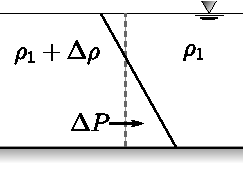
\includegraphics[width=0.46\textwidth, clip=true]{inertialAdjustment}
    & 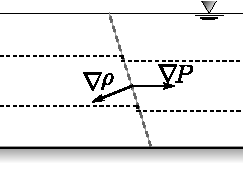
\includegraphics[width=0.46\textwidth, clip=true]{inertialAdjustmentb}

  \end{tabular}
\end{center}
\caption{
(a) Adjustment of a fluid subject to a horizontal difference in density
    in a non-rotating frame.
(b) Isopycnals and isobars (dashed lines), and the pressure and density
    gradient for a unstable condition.
        }
\label{f:drivedrag}
\end{figure}
%%% INCLUDE A FIGURE HERE  \ref{f:Marsigli}
%%%%%%%%%%%%%%%%%%%%%%%%%%%%%%%%%%%%%%%%%%%%%%%%%%%%%%%%%%%%%%%%%

The term responsible for the instability is quantified mathematically as
the curl between the density and pressure gradients, that is:
\beq
\nabla \rho \times \nabla p
\,,
\ee{solenoid}
as we will show in \refsect{s:vorticity}. Obviously, this definition
agrees with the intuitively notion we just developed.

Consider now a further complication, and think about what would happen if
the frame of reference were to be rotating in our previous experiment. In
that case we would have to consider the apparent forces that develop on
the individual fluid parcels of our flow, one proportional to the
position (the centrifugal acceleration) and other proportional to the
velocity (the Coriolis force) of each parcel. However, in geophysical
applications the former one is often unimportant\footnote{Due to the
departure from sphericity of the earth}\rf{Holton79}, and only the
effects of the Coriolis Force needs to be consider. Thus, if we repeat
our experiment from a initial state as before, the motion of the fluid
would be determined by the effects of the pressure gradient and the
Coriolis force.

In this new setup, each individual parcel starts moving due to the
pressure gradient force but the presence of rotation makes them deviate
from a straight trajectory; as Coriolis force acts at right
angles of the parcel velocity. Once these transient motions
disappear, an new balanced state is reached, where the velocity becomes
perpendicular to the pressure gradient force (see \reffig{f:GBalance}).
This balance state is referred commonly as geostrophic balance, and it
differs from the previous example in that in this new balance the
pressure gradient does not vanishes, but rather is balanced by the
Coriolis force. That is, from the inviscid, unforced Navier-Stokes
equations one would get:
\beq
\textbf{u}_g=-\frac{1}{f \rho} \textbf{k} \times \nabla_z p
\,,
\ee{Geostrophic}
where $\textbf{u}_g$ is the horizontal component of the velocity, $f$ is
the Coriolis parameter, $\rho$ is the density of the flow, $p$ is the
pressure and $g$ the acceleration due to gravity. In addition, the use of
the hydrostatic relation implies the following relation for the change in
the vertical; which is commonly referred as the thermal wind
equation\rf{Salmon98}:
    \PC{many of your equations are split into pieces - here is an example
    how to put the together, have a single citation to them, in this case
    \refeq{eq:TWE}}
\bea
\frac{\partial \rho u_g}{\partial p}
    &=& \frac{1}{f} \left(\frac{\partial \alpha}{\partial y}\right)
\continue
\frac{\partial \rho u_g}{\partial p}
    &=& -\frac{1}{f} \left(\frac{\partial \alpha}{\partial x}\right)
\,,
\label{eq:TWE}
\eea
where $\alpha$ is the specific volume of the fluid.

%%%%%%%%%%%%%%%%%%%%%%%%%%%%%%%%%%%%%%%%%%%%%%%%%%%%%%%%%%%%%%%%
\begin{figure}
\begin{center}
  % Requires \usepackage{graphicx}
  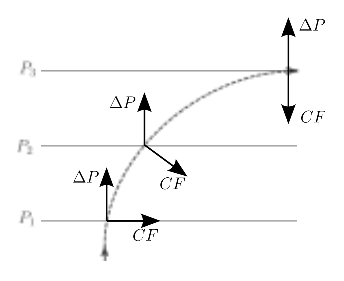
\includegraphics[width=0.5\textwidth, clip=true]{GeostrophicBalance}\\
\end{center}
  \caption{Process of geostrophic adjustment for an initially motionless fluid parcel.}
  \label{f:GBalance}
\end{figure}
%%% INCLUDE A FIGURE HERE  \ref{f:GBalance)
%%%%%%%%%%%%%%%%%%%%%%%%%%%%%%%%%%%%%%%%%%%%%%%%%%%%%%%%%%%%%%%%%

From the last relations, it is concluded that there is a equilibrium state,
 in the presence of rotation, where the isopycnals and
isobars are not necessarily parallel to each other. Nonetheless,
instability occurs when the isopycnal slope exceeds a critical value;
this type of phenomena is referred as baroclinic instability (see
\refref{Salmon98}).

But which are the stability
properties of this equilibrium, and the motions that generate afterwards?. The first of
this questions has been studied widely, and it uses linear approximations
to develop the relations between flow properties that need to be meet in
order for it to remain stable, or become unstable. The study of the motions that
develops after the initial instability is a more challenging problem as
nonlinear terms now become important. The hopes are that nonlinear theory
allow us to extract important knowledge about this phenomena even in high dimensional
simulations.

\section{Vorticity Equation}
\label{s:vorticity}

What is clear from Marsigli's experiment, is that the impact of the
solenoidal term is to induce vorticity in the fluid\footnote{The reader
is referred to \refref{kundu08} for an introductory, yet rigorous
treatment of vorticity. However, be aware that in Kundu's derivation of the
vorticity equation the density is not treated as a function of both
pressure and temperature, but only of pressure; so that the solenoidal
term is not considered.}. This variable is a fundamental property of the
fluid, and studying it has the power of greatly simplify the analysis of a
given flow. In fact, the first satisfactory attempts to model the atmosphere
where done by Charney considering the vorticity of quasigeostrophic flows.

Vorticity arises naturally from Navier-Stokes equations, and is just
a measure of the rotational speed of the fluid parcel. To make the
derivation explicitly, let's consider the inviscid equations of motion in
a rotating frame of reference\footnote{
    As explained in Section
    \ref{s:intro}, only the Coriolis' force ($\Omega \times \textbf{u}$) is
    considered in the equations, as the centripetal acceleration due to
    earths rotation can be ignored.
}, that is:
\beq
\frac{\partial \textbf{u}}{\partial t}+(\textbf{u} \cdot \nabla)\textbf{u}+2\Omega \times \textbf{u}
= -\frac{1}{\rho} \nabla p
\,.
\ee{NS1}
From vector calculus we note that:
\beq
(\textbf{u} \cdot \nabla)\textbf{u}=\frac{\nabla (\textbf{u} \cdot \textbf{u})}{2}- \textbf{u} \times \omega
\ee{VE0}
where $\omega$ is the vorticity. So that we can rewrite Navier-Stokes
equation in the following way:
\beq
\frac{\partial \textbf{u}}{\partial t}+(\omega+2\Omega) \times \textbf{u} = -\frac{1}{\rho} \nabla p -\frac{\textbf{u} \cdot \textbf{u}}{2}
\ee{NS2}
Taking the curl of this equation (noting that $\omega = \nabla \times
\textbf{u}$) gives:
\beq
\frac{\partial \omega}{\partial t}+\nabla \times ((\omega+2\Omega) \times \textbf{u}) = -\nabla \times\left(\frac{1}{\rho} \nabla p\right) -\nabla \times \frac{\textbf{u} \cdot \textbf{u}}{2}
\ee{VE1}
Finally using the identity $\nabla \times (A \times B) = A (\nabla
\cdot B)-B (\nabla \cdot A)+(B \cdot \nabla)A-(A \cdot \nabla)B$, the
chain rule for the pressure $\frac{1}{\rho} \nabla p = \nabla (p/\rho)-p
\nabla (1/\rho)$, and the fact that the curl of a gradient is zero, the
desired expression for the vorticity it is obtained from
\refeq{NS2} (see \refref{Salmon98}). That is:
\beq
\frac{d}{d t}\left(\frac{\omega_a}{\rho}\right)
=\left[\left(\frac{\omega_a}{\rho}\right) \cdot \nabla \right] \textbf{u}
  +\nabla p \times \nabla \left(\frac{1}{\rho}\right)
\ee{VE2}
where $\omega_a=\omega+2\Omega$ is the absolute vorticity. It is then
evident from this equations how the baroclinic term ($\nabla p \times
\nabla (1/\rho)$) can induce vorticity in the fluid by means of the
instabilities previously discussed.

Equation \refeq{VE2} can also be written for a single layer shallow water system as (see \refref{Vallis06}):
\beq
\frac{d}{dt}\left(\frac{\eta + f}{h}\right)=0
\,,
\ee{SW1}
where $\eta$ is the vertical component of the vorticity, $h$ the instantaneous depth of the fluid, and the quantity conserved is referred as potential vorticity ($q=(\eta + f)/h$). A generalization to two or  more layers is straight forward (see \refrefs{Vallis06,phillips51}).  Simplified form of this
expression, filtering unimportant motions for the large scale circulations
is developed next for a two layer system. However, the equations would be rich in dynamics as advection terms are retained for the horizontal
(so that a lot of interesting nonlinearities remains). Up to the date
there still much interesting features of this system to be studied.
    \SOA{I could include here a discussion about Kelvin circulation theorem,
    and how the baroclinic term would induce currents such as the sea breeze.
    However, I think I am extending a little to much in the basics. Hopefully
    this would make the project more readable.}




\section{2 Layer QG-Equations}
\label{s:qg}

If we intend to study baroclinic instability, we need to be able to
capture two basic properties of the flow (as shown in
\refsect{s:examples}): the nearly geostrophic motions of the fluid and
its vertical structure as given by \refeq{eq:TWE}. One of
the simplest mathematical systems that would capture this type of
behavior \refref{phillips51}, is a quasigeostrophic set of equations
discretized for two vertical layers. A quick derivation is given
here\footnote{
    We follow a intuitively approach for the sake of simplicity. However
    a much more systematic derivation can be made with asymptotic methods
    and the reader is advise to explore them (see for instance
    \refrefs{Vallis06, Majda03, Hasha05}), as they expose how different
    approximations relate to each other.
}. For in-depth derivations the  reader is referred to
\refrefs{Vallis06,Holton79,Salmon98,phillips51}.

%\item[2012-06-12 Sebastian to Predrag and Ashley]
%Do you ever define the model, draw a picture that says what is $x$ and what is $y$?
%If you do, refer to the place in the text it happens, and if you do not, define it in the
%text of your project (edit it freely, we can always update the ChaosBook.org posting by an
%improved version), and
%draw a clear picture what is what.
%
The geometry of the computational cell is sketched in \reffig{DomainDefinition}.
    \PC{2012-06-13 Predrag: incorporate/merge this into your writeup: ``
In this work, the baroclinic instability is modeled by a 2-layer
incompressible viscous fluid in a channel with no-slip side walls,
periodic in streamwise direction, top layer driven by `atmospheric
stream', \ie\ a constant total streamwise volume flow per unit time.
We impose uniform streamwise velocity of unit size, ignoring the
boundary condition (probably one should use a parabolic profile). With free slip the
layers are still unstable in the same way, just the boundary behavior is
different. Oceanographers prefer no-slip, perhaps because of coastal
stream. The bottom layer is not forced, no slip, no
\HREF{http://en.wikipedia.org/wiki/Ekman_layer}{Ekman layer}
(Ekman layer models friction at the bottom; that would make sense when
she works with 50 layers, but not two). The two layers are coupled by the
difference $\Phi_2 - \Phi_1$. Laplacian of stream function is vorticity.
Each layer is computed in terms of vorticity equations as a 2-dimensional
fluid. The lower layer has higher fluid density, and they are coupled
across their interface by difference of vorticity.

In our simulation this is about factor two; it is related to the
R\"osby deformation radius $L_R$. The spanwise $y$ width is $L_R/2\pi =
1/2$. Unless the width is larger than $L_R$, no instability. The
stream-wise aspect ration is about 8.
''
    }

\begin{figure}
  % Requires \usepackage{graphicx}
\begin{center}
  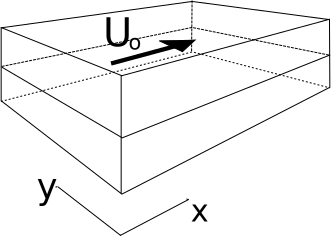
\includegraphics[width=0.4\textwidth]{DomainDefinition}\\
  \end{center}
  \caption{The geometry of the computational cell. Two layer quasigeostrophic model with vertical
  shear characterized by $U_o$, $x$ the streamwise, and $y$ the
  spanwise coordinate.
  The
geophysically relevant case is a channel whose zonal (streamwise) length is
substantially greater than its meridional (spanwise) breadth.
  }\label{DomainDefinition}
\end{figure}




%%%%%%%%%%%%%%%%%%%%%%%%%%%%%%%%%%%%%%%%%%%%%%%%%%%%%%%%%%%%%%%%
\begin{figure}[t]
\begin{center}
    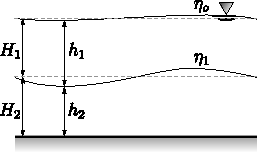
\includegraphics[width=0.6\textwidth, clip=true]{twolayermodel}
\end{center}
\caption{Two layer model considered in the simulations.}
\label{f:twolayer}
\end{figure}
%%%%%%%%%%%%%%%%%%%%%%%%%%%%%%%%%%%%%%%%%%%%%%%%%%%%%%%%%%%%%%%%%

Consider the situation in \reffig{f:twolayer}, where we have two layers of
different densities, equal depths $H$, and the Rossby number is small
enough so that we can use the quasi-geostrophic approximation. The
potential vorticity of each layer can then be written as:
\beq
q_i=\frac{\eta_i+f}{h_i}
\,,
\ee{PV}
where $\eta_i$ is the relative vorticity of each layer, $f$ the planetary
vorticity and $h_i$ distance between layers\footnote{
    We follow the derivation and the notation of \refref{Vallis06}
}. As we learned, this
property must be conserved by each layer, then:
\beq
\frac{d q_i}{dt}=\frac{d}{dt}\left(\frac{\eta_i+f}{h_i}\right)
   \simeq \frac{d}{dt}\left(f+\eta_i-f\frac{h_i'}{H_i}\right)=0
\,,
\ee{PVC}
where the approximation is only valid when Rossby number is small. $H_i$
is the unperturbed layer thickness, and $h_i'$ is the thickness
perturbation for layer $i$. Now let us introduce the geostrophic
equations to approximate the wind and the vorticity.

First note that from \refeq{Geostrophic} that the velocities only depend on the pressure gradient,
and that the fluid can be regarded as incompressible if we assume that the vertical gradient of $w$ is small.
Then the pressure will depend only depend on the height of the interfaces. An it can in turn be related to
$h_i$. That is, the height of the surfaces is given by:
\beq
\eta_o = h_1 + h_2 = h_1'+h_2'+2H
\ee{HS1}
\beq
\eta_1= h_2 = h_2' + H
\ee{HS2}
so that the pressure in the first layer is given by:
\beq
p = g \rho_1 (\eta_o-z)
\,,
\ee{Pre}
and the horizontal gradient is:
\beq
\nabla p = g \rho_1 \nabla \eta_o = g \rho_1 ( \nabla h_1' + \nabla h_2' )
\ee{Pre1}
With the same procedure it is found for the second layer:
\beq
\nabla p =  g \rho_1 ( \nabla h_1' + \nabla h_2' ) + g' \rho_1 \nabla h_2'
\,,
\ee{Pre2}
where $g'=(\rho_2-\rho_1)/\rho_1$ is the reduced gravity. The geostrophic condition then gives for the top layer:
\beq
u_g = -\frac{g}{f} \frac{\partial}{\partial y}(h_1'+h_2')
\ee{GEOS}
\beq
v_g = \frac{g}{f} \frac{\partial}{\partial x}(h_1'+h_2')
\,,
\ee{GEOS2}
and for the bottom layer:
\beq
u_g = -\frac{g}{f} \frac{\partial}{\partial y}(h_1'+h_2')-\frac{g'}{f} \frac{\partial h_2'}{\partial y}
\ee{GEOS3}
\beq
v_g = \frac{g}{f} \frac{\partial}{\partial x}(h_1'+h_2')+\frac{g'}{f} \frac{\partial h_2'}{\partial x}
\ee{GEOS4}

From the equations above, it is clear that the equations can be written
in terms of a stream function for each layer, such that $u_i=-\partial
\psi_i / \partial y$, $v_i=\partial \psi_i / \partial x$ and the
vorticity is simply written as $\eta_i = \nabla ^2 \psi$. The stream
functions being:
\beq
\psi _1 = \frac{g}{f} (h_1'+h_2')
\ee{SF1}
\beq
\psi _2= \frac{g}{f} (h_1'+h_2')+\frac{g' h_2'}{f}
\ee{SF2}

An expression for the potential vorticity of each layer in terms of the
stream functions, is obtained if we use these in \refeq{PVC}:
\beq
q_1=\beta y + \nabla^2 \psi_1 + \frac{f_o^2}{g'H}(\psi_2-\psi_1)-\frac{f_o^2}{gH}\psi_1
\ee{LE1}
\beq
q_2=\beta y + \nabla^2 \psi_2 + \frac{f_o^2}{g'H}(\psi_1-\psi_2)
\,,
\ee{LE2}
where the term $f_o^2 \psi_1/gH$ is much smaller than the others and can be dropped from the equations.

Note, that we now have a closed set of equation to solve. The equations
above are only dependent on $\psi_1$ and $\psi_2$, and as they are the
potential vorticity for each layer, they are exactly conserved ($d
q_i/dt=0$). Nonetheless, it is convenient to nondimensionalize the
variables; and we use the same scales as in \refref{Bracco03} for this
purposes. That is, we use $U$ for the characteristic velocity of the
flow, $L_R=(g'H)^{1/2}/f_o$ the internal Rossby deformation radius as the
horizontal scale, and $L_R/U$ for the time scale. This way,
\refeq{LE1} and \refeq{LE2} transform to:
\beq
q_1^*=\beta^* y + \nabla^2 \psi_1^* + F(\psi^*_2-\psi^*_1)
\ee{LEND1}
\beq
q^*_2=\beta^* y + \nabla^2 \psi_2^* + F(\psi^*_1-\psi^*_2)
\,,
\ee{LEND2}
where $\beta^*=\beta U / L_R^2$ and $F=f_o^2 L_R^2 /(g'H)$
    \SOA{I am not really sure if these is set to one in the simulations,
    however it is in \refref{Bracco03}
}. The superscript denotes a nondimensional variable and will be dropped
hereafter, writing above equations as:
\beq
q_1=\beta y + \nabla^2 \psi_1 + F(\psi_2-\psi_1)
\ee{LEND1a}
\beq
q_2=\beta y + \nabla^2 \psi_2 + F(\psi_1-\psi_2)
\ee{LEND2b}
Lastly, it is also convenient to introduce some sort of dissipation in the system. Linear drag can be added easily by considering the conservation equations for $q_i$ as in \refref{Bracco03}, that is:
\beq
\frac{d q_i}{dt}=\frac{\partial q_i}{\partial t}+J(\psi_i,q_i)=-\nu \nabla^2 \psi_i
\,,
\ee{Cons}
where $J(\psi,q)=\psi_x q_y - \psi_y q_x$ and $\nu$ is a nondimensional
viscosity coefficient. Equivalently this three las equations can be
rewritten as:
\begin{eqnarray}
\frac{\partial}{\partial t} \left(\nabla^2 \psi_1 + F(\psi_2-\psi_1)\right)+\textbf{u} \cdot \nabla \left(\nabla^2 \psi_1 + F(\psi_2-\psi_1)\right)+\beta \frac{\partial \psi_1}{\partial x} = -\nu \nabla^2 \psi_1 \nonumber \\
\frac{\partial}{\partial t} \left(\nabla^2 \psi_2 + F(\psi_1-\psi_2)\right)+\textbf{u} \cdot \nabla \left(\nabla^2 \psi_2 + F(\psi_1-\psi_2)\right)+\beta \frac{\partial \psi_2}{\partial x} =-\nu \nabla^2 \psi_2 \nonumber \\
 \label{LEND3}
\end{eqnarray}

The last two equations constitute a closed set for $\psi_1$ and $\psi_2$,
far more convenient than its dimensional form, as all terms are
scaled so that its magnitude is $O(1)$. We can now use this model as a
simplified version to study baroclinic instability. Nonlinear terms are retained, so that its dynamics still is rich and not
fully understand up to date.
%We begin by considering Boussinesq approximation to Navier-Stokes
%equations. This arise when the density variations are small compared to
%the absolute value of itself (as is often found in the ocean), and the
%equations are simplified by only retaining the effects of the changes of
%density for the gravity terms (see \refref{Vallis06}). The equations are:

\section{Stability Theory}
\label{s:stability}

As we seen in the previous chapter, geostrophy is an equilibrium state of the Navier-Stokes equations. It is now convenient to ask how stable this state is, that is, how much does the isopycnals need to slope in order for baroclinic instability to develop, or equivalently, how fast the winds must be. For this we assume a background state of the flow, linearize the equations of motion around this state, assume a sinusoidal form for the disturbances and extract stability coefficients from the analysis (i.e. a bifurfication analysis is performed). It is fair to say that this has been the most common approach when dealing with baroclinic instability. And there have been great studies which differ in their assumptions. Here we focus in the particular set of equations derived in the previous sections (commonly called the Philip problem). However, more general forms of this analysis exist, where the equations for a continuously stratified atmosphere are considered (for example in the Eady or the Charney problems).

It is also important to keep in mind the limitations of this kind of analysis. They are highly idealized as they consider linearized relationships around simple background flows. Nevertheless, they are indispensable to understand atmospheric and oceanic circulation

We follow the procedure outlined by Hasha\rf{Hasha05} or in a simpler
fashion in \refref{Salmon98}, as it is an elegant systematic approach
which borrows notation from quantum mechanics. First, assume a shear flow
with mean velocities $U$ in the upper layer and $-U$ in the lower one.
This implies that the stream functions can be computed as:
\begin{eqnarray}
\psi_1 = -U y + \psi_1' \nonumber \\
\psi_2 =  U y + \psi_2'
\label{psi_base}
\,,
\end{eqnarray}
where the primes denote perturbations around the mean state. Replacing this in \refeq{LEND3}, and ignoring the high order perturbation terms and viscous dissipation \SOA{I have ignored dissipation here so I think that the same results as in Vallis' should be obtained. However, notation is a bit different.}, one obtains:
\begin{eqnarray}
\left(\frac{\partial}{\partial t}+U \frac{\partial}{\partial x}\right)\left(\nabla^2 \psi_1 + F(\psi_2-\psi_1)\right) +\frac{\partial \psi_1}{\partial x}(\beta + 2FU) = 0 \nonumber \\
\left(\frac{\partial}{\partial t}+U \frac{\partial}{\partial x}\right)\left(\nabla^2 \psi_2 + F(\psi_1-\psi_2)\right) +\frac{\partial \psi_2}{\partial x}(\beta - 2FU) = 0 \nonumber \\
\label{model_eq}
\,,
\end{eqnarray}
where we have dropped the primes. This can be written in matrix form as:
\beq
\left(\frac{\partial}{\partial t} M - L\right) \Psi=0
\,,
\ee{MF1}
where
\begin{equation}
\begin{pmatrix}
  \nabla ^2 - F & F \\
  F & \nabla^2 - F \\
\end{pmatrix}
\label{Mmatrix}
\end{equation}
\begin{equation}
\begin{pmatrix}
  -U \frac{\partial}{\partial x}(\nabla ^2-F)-(\beta+2FU)\frac{\partial}{\partial x}
   & -U F \frac{\partial}{\partial x} \\
   U F \frac{\partial}{\partial x}
   & U \frac{\partial}{\partial x}(\nabla ^2-F)-(\beta-2FU)\frac{\partial}{\partial x}
\end{pmatrix}
\label{Mmatrix2}
\end{equation}
Seeking solutions of the form
\begin{equation}
\Psi (x,y,t)=\hat{\Psi} (k,m,U) e^{i(kx+my-\omega t)}
\,,
\label{PRT}
\end{equation}
where $k$, $m$ are the horizontal wave numbers and $\omega$ the frequency
of the perturbation, one obtains new matrixes $\hat{M}$ and $\hat{L}$ as
functions of this new variables (see \refref{Hasha05}), so that:
%    \SOA{This might be becoming a little to cryptic here. Do you think we
%    should expand on the procedure?}
\beq
\left( \hat{L}+i \omega \hat{M}\right) \Psi=0
\,.
\ee{MF2}
In order to have nontrivial solution the determinant of $\left( \hat{L}+i
\omega \hat{M}\right)$ must vanish, which gives a relation
for $\omega$ (i.e. the dispersion relationship for the
perturbations) and a critical velocity for the flow to be unstable.
However, in our specific case we would set $\beta =0$ so that the flow would always
be unstable.\footnote{Unless the domain is not wide enough for the instability to occur.}
%    \SOA{Currently making the calculations for this case, just to make
%    sure that I have the correct dispersion relationship. I don't know if
%    it is as easy as setting $r = 0$ in Hasha report. I was also thinking
%    about making the calculations considering the term $\nabla ^4 \eta$.
%    But probably is done somewhere else. Let me know if you think it is
%    important to do so.}
%\beq
%\omega = ...%-\frac{\beta k}{K^2}\frac{K^2+F}{K^2+2F} \pm \frac{\sqrt{k^2K^4(K^4-4F^2)U^2+F^2(\beta k)^2}}{K^2(K^2+2F)}
%\ee{Dis}
%the model is then unstable if $\omega$ has an imaginary component, which is only possible if:
%\beq
%%k^2K^4(K^4-4F^2)U^2+F^2(\beta k)^2<0
%\ee{condition}
%The critical velocity for the instability is then given by:
%\beq
%U_c=%\sqrt{\frac{F^2(\beta k)^2}{k^2K^4(K^4-4F^2)U^2}}
%\ee{condition}
Thinking in terms of \statesp\ for the dynamical system
\footnote{
    That is, decomposing the PDE of the flow into
    a series of ODE for the amplitude of the harmonics.
}
(see\refref{DasBuch}), what was has been done up to here, is to find an equilibrium point of
the system and analyze its bifurcations. This is no small task, and that
is the reason of the vast amount of literature published in the subject.
Now we are interested in what happens next. And we will try to analyze
this by making use of the symmetries of the flow.

\section{Nonlinear Theory}
\label{s:nonlinear}
\subsection{A New Framework}
At this point we have a good idea of what baroclinic instability is and how it has been commonly approached. Now we wish to move on and try to explore the dynamics described by our simplified model while retaining all nonlinear contributions.
We will need a smart way to solve our equations of motion, and an even smarter way to represent their solutions.

The first step is to think about our equations in a dynamical framework;
that is, in \statesp. Thus, writing the system as follows:
\beq
\frac{d X_i}{d t} = F(X_i)
\ee{DS}
where each $X_i$ correspond to a coordinate in this space. Clearly, not
the case of \refeq{NS1}, where $\textbf{u}$ is a dependent variable of
both space and time. Nonetheless, we can formulate it in this form by the
use of spectral methods expressing the velocity as:
\beq
\textbf{u}=\sum \widehat{u} \phi (\textbf{x})
\ee{DS2}
where $\phi$ are basis function defined for the entire
domain\footnote{This could be any set of orthogonal functions (i.e.
Fourier, Legendre or Chebyshev series)} and $\widehat{u}$ their
respective amplitudes. Substituting this in \refeq{NS2}, and using and
appropriate relationship to account for the pressure, we obtain a system
like \refeq{DS} for the amplitudes of the basis functions. That is:
\beq
\frac{d \widehat{u}_i}{d t} = G(\widehat{u}_i)
\ee{DS3}
system which can be relatively easily integrated.
    \PC{will believe it when I see the results}
It should be noted that the above is much more than just a convenient
method to solve the Navier-Stokes equations; it is a framework to study
continuum equations as dynamical systems. In \statesp, a point
represents a physical state of the full system, i.e. the three
dimensional velocity field. This implies that Navier-Stokes equations can
be thought as an infinite dimensional space where the harmonics represent
each dimension of it \footnote{This view is due to Hopf, who's insight on
turbulence where way ahead of his time; and have proven to be an
invaluable tool (see \refref{hopf48})}. However, the number of dimension
consider in practice is finite and limited either by the computer power
available, or the smallest scale one can actually solve. No long time ago
considering only a handful of dimensions was possible.
Nowadays, computer power is such that DNS\footnote{Direct Numerical
Simulations. The approach of this method is to solve Navier-Stoke
equations up to the scale where dissipation occurs and kinetic energy is
converted to heat.} are possible and considering 100,000 dimensions or
more is common for small domains.

But given the exuberant number of dimensions, how are we to visualize the
flows in \statesp? there is not need to panic about this, although
visualizations is challenging the important dynamics are embedded in
lower dimensional manifolds. This was first noted by Hopf, who speculated
that viscosity must lower the effective dimensions of the system. An
example would be a laminar flow which is embedded in a infinite space;
which due to its high viscosity is effectively represented by a single
point in this space (for instance see \refref{GHCW07}). In the case of a
turbulent flow invariant solutions (periodic orbits, \rpo s, equilibrium
points and traveling waves) are starting point for finding the lower
dimensional invariant manifolds to consider. These solutions are usually
unstable, which makes imperative the use of a search algorithm in order
to find them.

Nonetheless, their role in dynamics is of such importance (see
\refref{skeleton}) that these intrinsic difficulties should not
discourage us from seeking for them. For instance, invariant solutions can be thought to represent
the coherent structures that characterize turbulent dynamics (see
\refrefs{Christiansen96,Visw07b}). In this view, the system spends some
time in a neighbor near one of this solutions, then jumps to the next and
spends some time there until it jumps to another, and so on. What it is
most striking is that this cycles resemble closely turbulent
trajectories, and are hard to tell apart from them. In fact, the
measurable quantities of a system depend mostly on these invariant
solutions (see \refref{DasBuch}), so that finding them gives a better
understanding of the system. In this study we give the first steps towards
finding these solutions in a baroclinic instability model by showing a plausible way to reduce the symmetries of the system.

Reducing the symmetries greatly simplifies the search of this structures. As solution do not
wonder as much in the reduced state space. In this space, traveling waves
reduce to equilibrium points, relative periodic orbits to periodic orbits and equilibrium points
are conserved. Our tool of choice for this reduction is the method of slices. We are interested
in rotating all the solutions to a hyperplane which intersects all symmetry group tangents (see \refref{DasBuch} for details). For
this we impose the condition:
\beq
\frac{\partial}{\partial \gSpace} \norm{\ssp-\LieEl\slicep}^2 =0
\,,
\ee{mini}
where $\ssp$ is our vector in state space, $\gSpace$ the rotating frame
(i.e. the angle by which the solution is rotated) and $\slicep$ a
template representative of our local dynamics. Of course, our slice would
not be good for the entire manifold, and it is necessary to consider a
set of this slices in order to capture the entire dynamics of the system
\refref{atlas12}. More details of this will be given in the next section.

Once we are done with the slicing, the hope is that this makes it easier
to look for this invariant solutions. After all, the "dancing" solutions
have been settled to the slice. But first, we need to define them in a
quantitative manner so it is clear what we mean by invariant solutions.
First, let's think again in terms of physical space \refeq{NS2}. Note
that we can write the system as:
\begin{eqnarray}
\frac{\partial \textbf{u}}{\partial t}
=F(\textbf{u})
    \,,\quad
f^{t}(\textbf{u})=\textbf{u}+\int_{0}^{t}{F(\textbf{u}) d \tau}
\,,
\label{NS4}
\end{eqnarray}
thus, we are seeking solutions of the following form (as shown in \refref{GHCW07}):
\begin{eqnarray}
F(\textbf{u}_{EQ}) &=& 0 \continue
F(\textbf{u}_{TW}) &=& -c \cdot \nabla \textbf{u}_{TW} \continue
f^{T_p}(\textbf{u}_{p}) &=& u_p \continue
f^{T_p}(\textbf{u}_{p}) &=& u_p
\,,
\label{NS_Solutions}
\end{eqnarray}
    \SOA{I have to fix the second equation justification.}
where this represent respectively equilibrium points, relative
equilibrium points, periodic orbits and \rpo s.

Finally, note that one additionally aspect  one should care about is the
connection between these different solutions. That is, how is one to get
from one recurrent pattern to the other? Heteroclitic connections (i.e.
the trajectories which exactly connect invariant solutions; see for
instance \refref{GHCV08}), are commonly studied for this purposes as
these organize how the flow transits from one manifold to the next.

In this project, we limit ourselves to show how to make the slicing,
hoping this would encourage more in depth study of the subject. However,
we briefly discuss next how to start searching for the recurrences in the
system one the slicing is completed.

\subsection{Finding invariant solutions}

Finding invariant solution of a system with a high number of dimension is
not an easy task. And it is even harder if we do not reduce the
symmetries first. In doing so one is required to use a numerical method
to find them. However, due to the fact that huge Jacobian matrix would
have to be computed, implementing the Newton-Raphson standard search
method is not an option.
%Moreover, when other algorithms are used, the initial guess for the periodic orbit must be good enough so that the algorithm converges to the desired solution.

But not all hope is lost. Algorithms to find this structures have been
implemented and used successfully in a variety of simulations\SOA{Insert
references in the future)} (see for instance \refref{Visw07b}). This
methods depend on initial guesses of this periodic orbits, and there are
several approaches one can take to make the right ones. One of this
approaches is given in \refref{Visw07b}, where the rate of energy
dissipation and energy input for a system is computed based on the
velocity field, and then plotted together. This way the entire
multidimensional system is projected into two physical meaningful
dimensions and guesses are made based on approximate recurrences of the
traced curve.
    \SOA{FIGURE I will put her one of the figures of
        Viswanath's paper}

After reducing the symmetries, the next step would be to evaluate the
possibility of a periodic orbit based on the criteria discussed here.
%That is, to search for close recurrences of the flow based on two dimensional projections of the d-dimensional space.
However, we proceed one step at a time. So let us go back to reducing the
symmetry.

\subsection{Symmetry Reduction}
Up to here we have gather enough background to start making attempts to
reduce the symmetry. The system to consider is that of Section
\ref{s:qg}. And the code is the same as the one programmed by Bracco in
\refref{Bracco03}\footnote{Without bottom topography or beta effect.}.
The typical results of the simulation are shown in figure
\ref{f:fouriervort3}.

    \begin{figure}[t]
    \begin{center}
    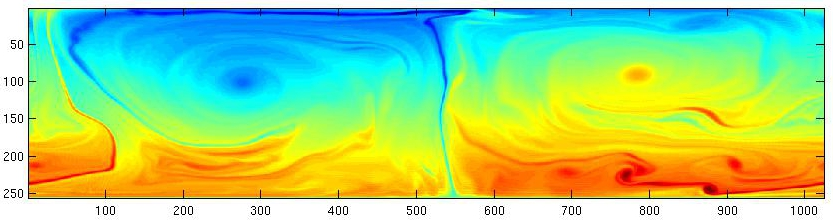
\includegraphics[width=0.9\textwidth, clip=true]{Vort_example}
    \end{center}
    \caption{Vorticity field ($\xi$) for the top layer in the model.}
    \label{f:fouriervort2}
    \end{figure}

The code makes uses a pseudo-spectral method to solve the nonlinear PDE
given in \ref{model_eq} but with $\beta=0$ and $\psi_2 =\psi_2'$. For
this, Fast Sine Transforms are used along the $y$ direction, and Fast
Fourier Transforms along the $x$ direction . This means that the
vorticity can be represented as:

    \begin{figure}[t]
    \begin{center}
    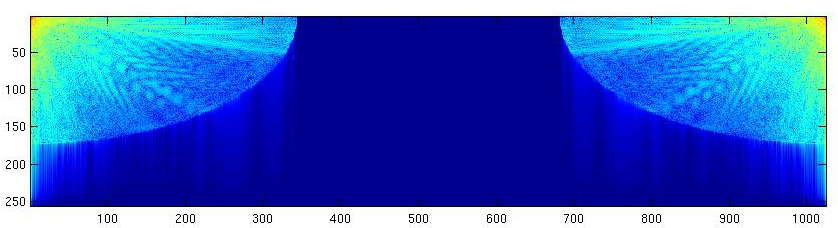
\includegraphics[width=0.9\textwidth, clip=true]{fourier_example}
    \end{center}
    \caption{Spectral representation of the vorticity field
    ($ln(1+abs(a_{lk}))$). Note that some frequencies are just the complex
    conjugate of others.}
    \label{f:fouriervort3}
    \end{figure}

    \beq
    \xi(x,y)=\sum_{k=0}^{N-1} a_{lk} e^{-2 i \pi k x/N}
    \ee{fft}

Additionally, the system has periodic boundaries along the $x$ axis, so
it has a continuous symmetry along this axis $\xi(x)=\xi(x+L_x)$; where
$L_x$ stands for the length of the domain. The one-parameter rotation
group acting on this variable, would be then given by (see
\refref{ACHKW11}):
\beq
\LieEl(\gSpace)=\textrm{diag}\{e^{-2 i \pi k \gSpace/N}\}
\ee{gpara}

When acting on a point in state space ($\LieEl(\gSpace) a$), the effect
of $\LieEl$ is to translate the solution along $x$ without changing any o
the properties of the simulation. Furthermore, in state space the group
orbit traces a trajectory which topologically is a circle, and the group
tangent of the circle at point $a$ is given by the derivative of
$\LieEl$:
\beq
\textbf{T}=\textrm{diag}\{-2 i \pi k /N\}
\ee{gpara2}

Now, to reduce the symmetry, we select a template representative our our
physical simulation (the slice $a'$), and seek for the rotating frame
$\gSpace(t)$ that continually rotates a trajectory back to the slice.
This, by making use of condition \ref{mini}. Care is taken as we are
dealing with complex vectors, so that the norm represents the
multiplication of a vector with its conjugate transform. That is,
starting with:
\beq
\frac{\partial}{\partial \gSpace} \norm{\ssp-\LieEl\slicep}^2 =0
\,,
\ee{min2}
expanding, simplifying and noting that $\Re(\ssp^\dagger \Lg \ssp)=0$ one
arrives at the slicing condition:
\beq
    \Re(\sspRed^\dagger \Lg \slicep)=0
\ee{min3}
which is a similar condition to the one obtained for real cases.
Translating it into a somewhat more implementable equation gives:
\beq
    \Re(\sspRed^\dagger \Lg \slicep)=
    \Re\left(\frac{-2 \pi i}{N} \sum_{k=0}^{N-1} \sum_{k=0}^{M-1}
    \overline{a_{lk}} a'_{lk} k e^{\frac{-2 \pi i k}{N} \gSpace}
        \right)=0
\ee{min4}
Now we are all set to seek for this solutions. A Newton-Raphson, or
similar, seeking method can be implemented by using
$F(\gSpace)=\Re(\sspRed^\dagger \Lg \slicep)$ and
$F'(\gSpace)=\frac{\partial}{\partial \gSpace}\Re(\sspRed^\dagger \Lg
\slicep)$ for each time step. Effort are being carried right now to
implement this algorithm, however for the time being we only provide the
methodology.


    \ifboyscout
    \PC{insert from
        \HREF{../atlas/atlas12.pdf}{Chaos Gang paper}, rewrite}
The {\template} $\slicep$ should be a generic \statesp\ point in the
sense that its group orbit has the full dimension of the group
\Group. The set of the group orbit points {closest} to the
\template\ \slicep\ forms a neighborhood of \slicep\ in which each group
orbit intersects the hyperplane \emph{only once}. A \slice\ hyperplane
captures neighboring group orbits until, for a point $\sspRSing$ not so
close to the \template, the group tangent vector $t(\sspRSing)$ lies in
the \slice\ hyperplane. The group orbits for such points are grazed
tangentially rather than sliced transversally, much like what happens at
the \poincBord\ for evolution in time.
This is also a linear condition and defines the \chartBord\ ${\cal
S}$,\rf{SiCvi10,FrCv11} a $(d\!-\!2)$\dmn\ manifold, which contains
all the points $\sspRSing$ whose group tangents lie in the \slice\
hyperplane, \ie,
\beq
\braket{\sspRSing}{\sliceTan{}} \,=\, 0
      \mbox{ and }
\braket{\groupTan(\sspRSing)}{\sliceTan{}} \,=\, 0
\,.
\label{sliceSingl0}
\eeq
${\cal S}$ also contains all points for which $\groupTan(\sspRSing)=0$.
While for the \PoincSec s the analogous points were \eqva\ (captured only
if the section cut through them), for \slice\ hyperplanes points with
vanishing group actions belong to invariant subspaces, and, by its
definition, every {\chartBord} automatically includes \emph{all}
invariant subspaces.

The norm square of a tangent vector is given by
\beq
\Norm{\groupTan(\ssp)}^2
    = - \braket{\groupTan(\ssp)}{\groupTan(\ssp)}
    = \frac{2 \pi}{N} \sum_{k=0}^{N-1} \sum_{k=0}^{M-1}
       k^2 \, \overline{a_{lk}} a_{lk}
\ee{min5}
The product of the two tangents in \refeq{min4} is weighted by the
\SOn{2} quadratic Casimir
    \PC{I have not checked \refeq{min4}, \refeq{min5} and/or \refeq{min6}}
\beq
    - \Re(\sspRed^\dagger \Lg^2 \slicep)=
    \Re\left(\frac{-2 \pi i}{N} \sum_{k=0}^{N-1} \sum_{k=0}^{M-1}
    \overline{a_{lk}} a'_{lk} k^2 e^{\frac{-2 \pi i k}{N} \gSpace}
        \right)
\,
\ee{min6}

    \fi % end \ifboyscout

\section{Acknowledgments}
The author would like to acknowledge the valuable discussions and advicse
obtained during the course of the semester from Professors Predrag
Cvitanovi{\'c}, Annalisa Bracco and Peter J. Webster, as well as the
students and researchers that attended the Spring 2012  "PHY-7224
Nonlinear Dynamics". This was a very enjoyable and enlightening
experience.


%\section{Invariant Solutions in the nonlinear baroclinic stability model}
%\label{s:model}
